% MẪU TỔNG HỢP KHO DỮ LIỆU TIKZ CHO LATEXTOPIC
% File này dùng để gom nhóm, kiểm tra và quy hoạch cấu trúc trước khi code Tool
% -----------------------------------------------------------------------------
\documentclass[12pt,a4paper,oneside]{book}
\usepackage{fouriernc}
\usepackage{amsmath,amssymb}
\usepackage{tikz,tkz-tab,tkz-euclide,pgfplots}
\usepackage[top=1.5cm, bottom=1.5cm, left=1.2cm, right=1.2cm] {geometry}
\usepackage[dethi]{ex_test}

% Khai báo thư viện tcolorbox để kẻ khung mã source code
\usepackage[many,most]{tcolorbox}
\tcbuselibrary{listings}

\begin{document}
\Opensolutionfile{ans}

\begin{center}
    \LARGE \textbf{KHO MẪU HÌNH VẼ TIKZ - PHÂN LỚP QUẢN LÝ}
\end{center}

\vspace{1cm}
% =========================================================================
% VÙNG 1: CÁC MẪU GỐC HOÀN CHỈNH (MAIN TEMPLATES)
% (Giữ nguyên cấu trúc/tọa độ từ vốn ban đầu của file KyThuatVeNhanhCodeTeX)
% =========================================================================
\section*{VÙNG 1: MẪU GỐC CHUẨN (KHÔNG CHỈNH SỬA)}

\subsection*{1.1. Chóp tam giác có cạnh bên vuông góc với đáy (SA = h)}

\noindent
\begin{minipage}[c]{0.45\textwidth}
\centering
\begin{tikzpicture}[scale=1,>=stealth, font=\footnotesize, line join=round, line cap=round]
	\tkzDefPoints{0/0/A,1.2/-1.5/B,4/0/C}
	\coordinate (S) at ($(A)+(0,3)$);
	\tkzDrawPolygon(S,A,B,C)
	\tkzDrawSegments(S,B)
	\tkzDrawSegments[dashed](A,C)
	\tkzDrawPoints[fill=black,size=4](A,B,C,S)
	\tkzMarkRightAngles[size=0.16](S,A,B S,A,C)
	\tkzLabelPoints[above](S)
	\tkzLabelPoints[below](B)
	\tkzLabelPoints[left](A)
	\tkzLabelPoints[right](C)
\end{tikzpicture}
\end{minipage}\hfill
\begin{minipage}[c]{0.52\textwidth}
\begin{tcolorbox}[colback=gray!5,colframe=blue!60!black,boxrule=1pt,arc=3pt,title=Code TikZ,left=2mm,right=2mm,top=1mm,bottom=1mm]
\scriptsize
\begin{verbatim}
\begin{tikzpicture}[scale=1,>=stealth,
    font=\footnotesize, 
    line join=round, line cap=round]
  \tkzDefPoints{0/0/A,1.2/-1.5/B,4/0/C}
  \coordinate (S) at ($(A)+(0,3)$);
  \tkzDrawPolygon(S,A,B,C)
  \tkzDrawSegments(S,B)
  \tkzDrawSegments[dashed](A,C)
  \tkzDrawPoints[fill=black,size=4](A,B,C,S)
  \tkzMarkRightAngles[size=0.16](S,A,B S,A,C)
  \tkzLabelPoints[above](S)
  \tkzLabelPoints[below](B)
  \tkzLabelPoints[left](A)
  \tkzLabelPoints[right](C)
\end{tikzpicture}
\end{verbatim}
\end{tcolorbox}
\end{minipage}

\vspace{0.5cm}
\subsection*{1.2. Hình nón cơ bản}

\noindent
\begin{minipage}[c]{0.45\textwidth}
\centering
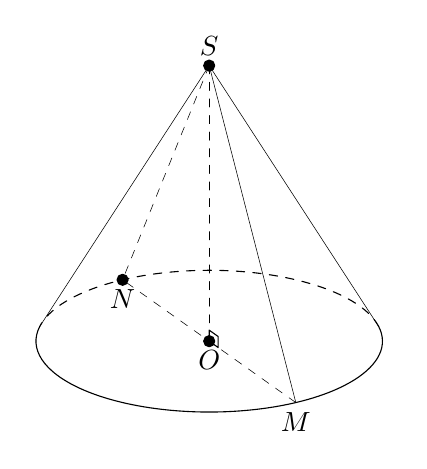
\begin{tikzpicture}[scale=1,>=stealth, font=\footnotesize, line join=round, line cap=round]
	\def \x{2.2} \def \y{0.9} \def \h{3.5}
	\coordinate (O) at (0,0);
	\coordinate (S) at ($(O)+(0,\h)$);
	\coordinate (M) at (-60:\x cm and \y cm);
	\coordinate (N) at ($(O)!-1!(M)$);
	\coordinate (l) at (168:\x cm and \y cm);
	\coordinate (r) at (12:\x cm and \y cm);
	\draw[dashed] (r) arc (12:168:\x cm and \y cm);
	\draw (r) arc (12:-192:\x cm and \y cm);
	\tkzDrawSegments(S,l S,r S,M)
	\tkzDrawSegments[dashed](S,O M,N S,N)
	\tkzDrawPoints[fill=black,size=4](O,S,N)
	\tkzLabelPoints[above](S);
	\tkzLabelPoints[below](O,M,N);
	\tkzMarkRightAngles[size=0.14](S,O,M)
\end{tikzpicture}
\end{minipage}\hfill
\begin{minipage}[c]{0.52\textwidth}
\begin{tcolorbox}[colback=gray!5,colframe=blue!60!black,boxrule=1pt,arc=3pt,title=Code TikZ,left=2mm,right=2mm,top=1mm,bottom=1mm]
\scriptsize
\begin{verbatim}
\begin{tikzpicture}[scale=1...]
  \def \x{2.2} \def \y{0.9} \def \h{3.5}
  \coordinate (O) at (0,0);
  \coordinate (S) at ($(O)+(0,\h)$);
  \coordinate (M) at (-60:\x cm and \y cm);
  ...
  \draw[dashed] (r) arc (12:168:\x cm and \y cm);
  \draw (r) arc (12:-192:\x cm and \y cm);
  \tkzDrawSegments(S,l S,r S,M)
  \tkzDrawSegments[dashed](S,O M,N S,N)
  \tkzDrawPoints[fill=black,size=4](O,S,N)
  \tkzLabelPoints[above](S);
  \tkzLabelPoints[below](O,M,N);
  \tkzMarkRightAngles[size=0.14](S,O,M)
\end{tikzpicture}
\end{verbatim}
\end{tcolorbox}
\end{minipage}

\vspace{1cm}
% =========================================================================
% VÙNG 2: MẪU PHÁT TRIỂN / TỔ HỢP (BIẾN THỂ TỪ MẪU GỐC)
% (Sử dụng gốc tọa độ phía trên, nhưng cắm thêm Add-ons: màu, góc, chi tiết phụ)
% =========================================================================
\section*{VÙNG 2: MẪU PHÁT TRIỂN \& TỔ HỢP (DỰ KIẾN)}

\subsection*{2.1. Biến thể: Chóp tam giác vuông + Tô đáy + Đánh dấu góc}

\noindent
\begin{minipage}[c]{0.45\textwidth}
\centering
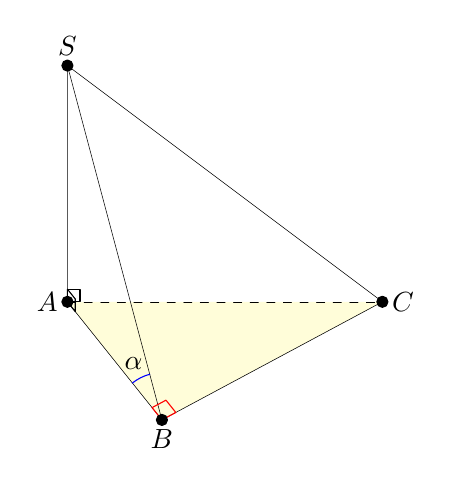
\begin{tikzpicture}[scale=1,>=stealth, font=\footnotesize, line join=round, line cap=round]
	% [Khung xương - Layer 1]
	\tkzDefPoints{0/0/A,1.2/-1.5/B,4/0/C}
	\coordinate (S) at ($(A)+(0,3)$);
	
	% [Add-ons: Tô màu đáy trước khi vẽ viền - Layer 2.1]
	\tkzFillPolygon[color=yellow!30, fill opacity=0.5](A,B,C)
	
	% [Khung hình gốc - Layer 2]
	\tkzDrawPolygon(S,A,B,C)
	\tkzDrawSegments(S,B)
	\tkzDrawSegments[dashed](A,C)
	
	% [Add-ons: Đánh dấu góc & Cạnh bằng nhau - Layer 3]
	\tkzMarkRightAngles[size=0.16](S,A,B S,A,C)
	\tkzMarkRightAngles[size=0.2,color=red](A,B,C) % Vuông tại đáy B
	\tkzMarkAngles[size=0.6cm,arc=l,color=blue](S,B,A) % Góc SB và đáy
	\tkzLabelAngles[pos=0.8](S,B,A){$\alpha$}
	
	% [Nhãn - Layer 4]
	\tkzDrawPoints[fill=black,size=4](A,B,C,S)
	\tkzLabelPoints[above](S)
	\tkzLabelPoints[below](B)
	\tkzLabelPoints[left](A)
	\tkzLabelPoints[right](C)
\end{tikzpicture}
\end{minipage}\hfill
\begin{minipage}[c]{0.52\textwidth}
\begin{tcolorbox}[colback=gray!5,colframe=red!60!black,boxrule=1pt,arc=3pt,title=Code Tổ hợp Modun,left=2mm,right=2mm,top=1mm,bottom=1mm]
\scriptsize
\begin{verbatim}
\begin{tikzpicture}[scale=1...]
  % Khung xương - Layer 1
  \tkzDefPoints{0/0/A,1.2/-1.5/B,4/0/C}
  \coordinate (S) at ($(A)+(0,3)$);
  
  % Add-ons: Tô đáy
  \tkzFillPolygon[color=yellow!30, 
    fill opacity=0.5](A,B,C)
  ... Vẽ Khung viền ...

  % Add-ons: Đánh dấu góc
  \tkzMarkRightAngles[size=0.16](S,A,B S,A,C)
  \tkzMarkRightAngles[size=0.2,color=red](A,B,C)
  \tkzMarkAngles[size=0.6cm,arc=l,
    color=blue](S,B,A)
  \tkzLabelAngles[pos=0.8](S,B,A){$\alpha$}
  ...
\end{tikzpicture}
\end{verbatim}
\end{tcolorbox}
\end{minipage}

\vspace{0.5cm}
\subsection*{2.2. Biến thể Đồ thị: Parabol + Miền diện tích (Tích phân Area)}

\noindent
\begin{minipage}[c]{0.45\textwidth}
\centering
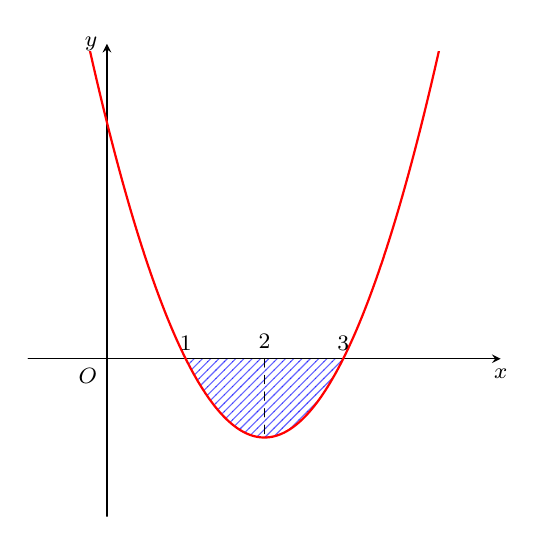
\begin{tikzpicture}[scale=1,>=stealth, font=\footnotesize, line join=round, line cap=round]
	\def\a{1} \def\b{-4} \def\c{3} 
	\def\xmin{-1} \def\xmax{5}
	\def\ymin{-2} \def\ymax{4}
	
	% [Add-on: Tô miền kẹp giữa trục hoành và hàm (S)]
	\fill[pattern=north east lines,opacity=0.6, pattern color=blue] plot[domain=1:3](\x,{\a*(\x)^2+\b*(\x)+\c}) -- (3,0) -- (1,0) -- cycle;

	% [Khung hệ trục]
	\draw[->] (\xmin,0)--(\xmax,0) node [below]{$x$};
	\draw[->] (0,\ymin)--(0,\ymax) node [left]{$y$};
	\node at (0,0) [below left]{$O$};
	
	% [Khung đồ thị gốc]
	\clip (\xmin+0.1,\ymin+0.1) rectangle (\xmax-0.5,\ymax-0.1);
	\draw[smooth,samples=300,thick,color=red] plot(\x,{\a*(\x)^2+\b*(\x)+\c});
	
	% [Chữ giải tích Add-ons]
	\draw[dashed, thin] (2,0) node[above]{$2$} -- (2,-1); % Tọa độ đỉnh
	\node at (1,0.2) {$1$};
	\node at (3,0.2) {$3$};
\end{tikzpicture}
\end{minipage}\hfill
\begin{minipage}[c]{0.52\textwidth}
\begin{tcolorbox}[colback=gray!5,colframe=red!60!black,boxrule=1pt,arc=3pt,title=Code Tổ hợp Modun,left=2mm,right=2mm,top=1mm,bottom=1mm]
\scriptsize
\begin{verbatim}
\begin{tikzpicture}[scale=1...]
  \def\a{1} \def\b{-4} \def\c{3} 
  \def\xmin{-1} \def\xmax{5}
  
  % Add-on: Tô diện tích Tích phân
  \fill[pattern=north east lines,opacity=0.6, 
   pattern color=blue] 
   plot[domain=1:3](\x,{\a*(\x)^2+\b*(\x)+\c}) 
   -- (3,0) -- (1,0) -- cycle;

  ... Vẽ khung trục tọa độ ...
  ... Cắt Viền (Clip) và Vẽ Parabol ...

  % Kéo tọa độ đỉnh  
  \draw[dashed, thin] (2,0) 
    node[above]{$2$} -- (2,-1);
  \node at (1,0.2) {$1$};
  \node at (3,0.2) {$3$};
\end{tikzpicture}
\end{verbatim}
\end{tcolorbox}
\end{minipage}

\Closesolutionfile{ans}
\end{document}